\documentclass[border=2pt]{standalone}
\usepackage{pgfplots}
\usepackage{xcolor}

\pgfplotsset{compat=1.18}

\definecolor{Garnet}{HTML}{73000A}
\definecolor{Gray10}{gray}{0.10}
\definecolor{Gray30}{gray}{0.30}
\definecolor{Gray50}{gray}{0.50}
\definecolor{Gray70}{gray}{0.70}
\definecolor{Gray90}{gray}{0.90}

\pgfplotsset{
  every axis/.style={
    axis line style={draw=black, line width=0.6pt},
    tick style={draw=black, line width=0.6pt},
    tick label style={font=\footnotesize\color{black}},
    label style={font=\small\color{black}},
    grid=both,
    grid style={draw=Gray90, line width=0.3pt},
    legend style={
      draw=none,
      font=\footnotesize\color{black},
      fill=white,
      at={(0.95,0.05)},
      anchor=south east,
    },
  },
  linestyle/.style={
    line width=0.8pt,
    mark=none,
  },
}
\begin{document}


% MS-DETR mAP50
\begin{figure}[h]
\centering
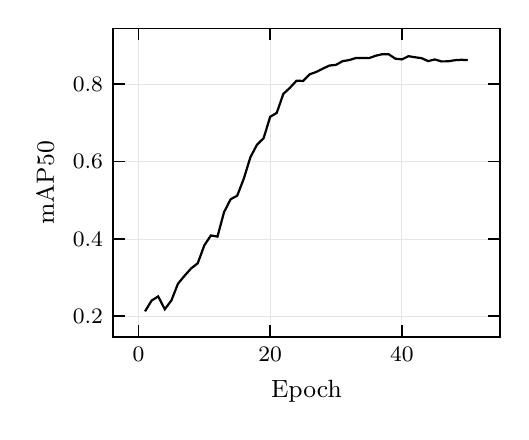
\begin{tikzpicture}
\begin{axis}[
  xlabel={Epoch},
  ylabel={mAP50},
  width=6.5cm,
  height=5.5cm,
]
\addplot[linestyle, color=black] coordinates {
  (1,0.212895)
  (2,0.240756)
  (3,0.251423)
  (4,0.218370)
  (5,0.240891)
  (6,0.284274)
  (7,0.304827)
  (8,0.323837)
  (9,0.336978)
  (10,0.383304)
  (11,0.409012)
  (12,0.406069)
  (13,0.469386)
  (14,0.502586)
  (15,0.511751)
  (16,0.556011)
  (17,0.611272)
  (18,0.643446)
  (19,0.660151)
  (20,0.715515)
  (21,0.725795)
  (22,0.774735)
  (23,0.790611)
  (24,0.808794)
  (25,0.808301)
  (26,0.825436)
  (27,0.831463)
  (28,0.840124)
  (29,0.848046)
  (30,0.849850)
  (31,0.859435)
  (32,0.862186)
  (33,0.867487)
  (34,0.867645)
  (35,0.867207)
  (36,0.873267)
  (37,0.877343)
  (38,0.877268)
  (39,0.865892)
  (40,0.863929)
  (41,0.872283)
  (42,0.869446)
  (43,0.867027)
  (44,0.859530)
  (45,0.863848)
  (46,0.858788)
  (47,0.858940)
  (48,0.861785)
  (49,0.862955)
  (50,0.861994)
};
\end{axis}
\end{tikzpicture}
\end{figure}

% MS-DETR mAP50-95
\begin{figure}[h]
\centering
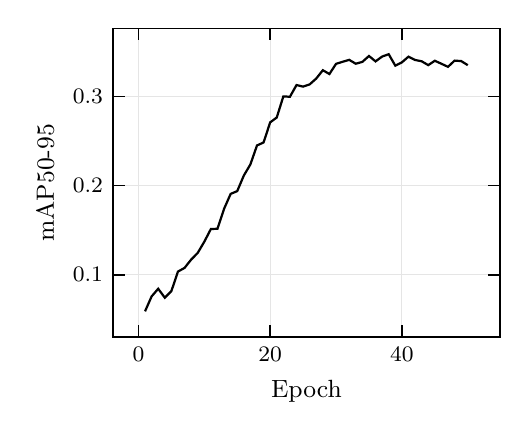
\begin{tikzpicture}
\begin{axis}[
  xlabel={Epoch},
  ylabel={mAP50-95},
  width=6.5cm,
  height=5.5cm,
]
\addplot[linestyle, color=black] coordinates {
  (1,0.058952)
  (2,0.075678)
  (3,0.084270)
  (4,0.074265)
  (5,0.081659)
  (6,0.103529)
  (7,0.107640)
  (8,0.116946)
  (9,0.124491)
  (10,0.137044)
  (11,0.151307)
  (12,0.151549)
  (13,0.173963)
  (14,0.190686)
  (15,0.193837)
  (16,0.211263)
  (17,0.223809)
  (18,0.245051)
  (19,0.248393)
  (20,0.270930)
  (21,0.276391)
  (22,0.300070)
  (23,0.299663)
  (24,0.312832)
  (25,0.311034)
  (26,0.313570)
  (27,0.320147)
  (28,0.329434)
  (29,0.325178)
  (30,0.336590)
  (31,0.338917)
  (32,0.341070)
  (33,0.336732)
  (34,0.338797)
  (35,0.345415)
  (36,0.339364)
  (37,0.344771)
  (38,0.347403)
  (39,0.334553)
  (40,0.338287)
  (41,0.344661)
  (42,0.340925)
  (43,0.339484)
  (44,0.335176)
  (45,0.340063)
  (46,0.336694)
  (47,0.333259)
  (48,0.340205)
  (49,0.339721)
  (50,0.335133)
};
\end{axis}
\end{tikzpicture}
\end{figure}



\end{document}
